\documentclass[11pt,preprint, authoryear]{elsarticle}

\usepackage{lmodern}
%%%% My spacing
\usepackage{setspace}
\setstretch{1.2}
\DeclareMathSizes{12}{14}{10}{10}

% Wrap around which gives all figures included the [H] command, or places it "here". This can be tedious to code in Rmarkdown.
\usepackage{float}
\let\origfigure\figure
\let\endorigfigure\endfigure
\renewenvironment{figure}[1][2] {
    \expandafter\origfigure\expandafter[H]
} {
    \endorigfigure
}

\let\origtable\table
\let\endorigtable\endtable
\renewenvironment{table}[1][2] {
    \expandafter\origtable\expandafter[H]
} {
    \endorigtable
}


\usepackage{ifxetex,ifluatex}
\usepackage{fixltx2e} % provides \textsubscript
\ifnum 0\ifxetex 1\fi\ifluatex 1\fi=0 % if pdftex
  \usepackage[T1]{fontenc}
  \usepackage[utf8]{inputenc}
\else % if luatex or xelatex
  \ifxetex
    \usepackage{mathspec}
    \usepackage{xltxtra,xunicode}
  \else
    \usepackage{fontspec}
  \fi
  \defaultfontfeatures{Mapping=tex-text,Scale=MatchLowercase}
  \newcommand{\euro}{€}
\fi

\usepackage{amssymb, amsmath, amsthm, amsfonts}

\def\bibsection{\section*{References}} %%% Make "References" appear before bibliography


\usepackage[round]{natbib}

\usepackage{longtable}
\usepackage[margin=2.3cm,bottom=2cm,top=2.5cm, includefoot]{geometry}
\usepackage{fancyhdr}
\usepackage[bottom, hang, flushmargin]{footmisc}
\usepackage{graphicx}
\numberwithin{equation}{section}
\numberwithin{figure}{section}
\numberwithin{table}{section}
\setlength{\parindent}{0cm}
\setlength{\parskip}{1.3ex plus 0.5ex minus 0.3ex}
\usepackage{textcomp}
\renewcommand{\headrulewidth}{0pt}
\renewcommand{\footrulewidth}{0.3pt}

\usepackage{array}
\newcolumntype{x}[1]{>{\centering\arraybackslash\hspace{0pt}}p{#1}}

%%%%  Remove the "preprint submitted to" part. Don't worry about this either, it just looks better without it:
\makeatletter
\def\ps@pprintTitle{%
  \let\@oddhead\@empty
  \let\@evenhead\@empty
  \let\@oddfoot\@empty
  \let\@evenfoot\@oddfoot
}
\makeatother

 \def\tightlist{} % This allows for subbullets!

\usepackage{hyperref}
\hypersetup{breaklinks=true,
            bookmarks=true,
            colorlinks=true,
            citecolor=blue,
            urlcolor=blue,
            linkcolor=blue,
            pdfborder={0 0 0}}


% The following packages allow huxtable to work:
\usepackage{siunitx}
\usepackage{multirow}
\usepackage{hhline}
\usepackage{calc}
\usepackage{tabularx}
\usepackage{booktabs}
\usepackage{caption}


\newenvironment{columns}[1][]{}{}

\newenvironment{column}[1]{\begin{minipage}{#1}\ignorespaces}{%
\end{minipage}
\ifhmode\unskip\fi
\aftergroup\useignorespacesandallpars}

\def\useignorespacesandallpars#1\ignorespaces\fi{%
#1\fi\ignorespacesandallpars}

\makeatletter
\def\ignorespacesandallpars{%
  \@ifnextchar\par
    {\expandafter\ignorespacesandallpars\@gobble}%
    {}%
}
\makeatother

\newlength{\cslhangindent}
\setlength{\cslhangindent}{1.5em}
\newenvironment{CSLReferences}%
  {\setlength{\parindent}{0pt}%
  \everypar{\setlength{\hangindent}{\cslhangindent}}\ignorespaces}%
  {\par}


\urlstyle{same}  % don't use monospace font for urls
\setlength{\parindent}{0pt}
\setlength{\parskip}{6pt plus 2pt minus 1pt}
\setlength{\emergencystretch}{3em}  % prevent overfull lines
\setcounter{secnumdepth}{5}

%%% Use protect on footnotes to avoid problems with footnotes in titles
\let\rmarkdownfootnote\footnote%
\def\footnote{\protect\rmarkdownfootnote}
\IfFileExists{upquote.sty}{\usepackage{upquote}}{}

%%% Include extra packages specified by user
\usepackage{booktabs}
\usepackage{longtable}
\usepackage{array}
\usepackage{multirow}
\usepackage{wrapfig}
\usepackage{float}
\usepackage{colortbl}
\usepackage{pdflscape}
\usepackage{tabu}
\usepackage{threeparttable}
\usepackage{threeparttablex}
\usepackage[normalem]{ulem}
\usepackage{makecell}
\usepackage{xcolor}
\usepackage{caption}
\usepackage{graphicx}
\usepackage{siunitx}
\usepackage{hhline}
\usepackage{calc}
\usepackage{tabularx}
\usepackage{adjustbox}
\usepackage{hyperref}

%%% Hard setting column skips for reports - this ensures greater consistency and control over the length settings in the document.
%% page layout
%% paragraphs
\setlength{\baselineskip}{12pt plus 0pt minus 0pt}
\setlength{\parskip}{12pt plus 0pt minus 0pt}
\setlength{\parindent}{0pt plus 0pt minus 0pt}
%% floats
\setlength{\floatsep}{12pt plus 0 pt minus 0pt}
\setlength{\textfloatsep}{20pt plus 0pt minus 0pt}
\setlength{\intextsep}{14pt plus 0pt minus 0pt}
\setlength{\dbltextfloatsep}{20pt plus 0pt minus 0pt}
\setlength{\dblfloatsep}{14pt plus 0pt minus 0pt}
%% maths
\setlength{\abovedisplayskip}{12pt plus 0pt minus 0pt}
\setlength{\belowdisplayskip}{12pt plus 0pt minus 0pt}
%% lists
\setlength{\topsep}{10pt plus 0pt minus 0pt}
\setlength{\partopsep}{3pt plus 0pt minus 0pt}
\setlength{\itemsep}{5pt plus 0pt minus 0pt}
\setlength{\labelsep}{8mm plus 0mm minus 0mm}
\setlength{\parsep}{\the\parskip}
\setlength{\listparindent}{\the\parindent}
%% verbatim
\setlength{\fboxsep}{5pt plus 0pt minus 0pt}



\begin{document}



\begin{frontmatter}  %

\title{Covariance Matrix Estimation via Macroeconomic Factor Modeling}

% Set to FALSE if wanting to remove title (for submission)




\author[Add1]{Tiago Baltazar (19776209)}
\ead{tiagobaltazar15@gmail.com}





\address[Add1]{Stellenbosch University, Western Cape, South Africa}


\begin{abstract}
\small{
This report compares the performance of two asset allocation strategies
namely; Risk Parity and Mean Variance during periods of volatility in
South Africa. Using South African financial data, the risk adjusted and
information ratio of a unleverd Risk Parity Index porfolio and Tangency
Index porfolio are compared. The research paper found that the Mean
Variance Optimisation approach is an superior asset allocation strategy
during periods of high volatility in South Africa.
}
\end{abstract}

\vspace{1cm}


\begin{keyword}
\footnotesize{
Asset Allocation \sep Risk Parity \sep Mean Variance Optimisation
\sep Volatility \\
\vspace{0.3cm}
}
\end{keyword}



\vspace{0.5cm}

\end{frontmatter}



%________________________
% Header and Footers
%%%%%%%%%%%%%%%%%%%%%%%%%%%%%%%%%
\pagestyle{fancy}
\chead{}
\rhead{19776209}
\lfoot{}
\rfoot{\footnotesize Page \thepage}
\lhead{\leftmark}
%\rfoot{\footnotesize Page \thepage } % "e.g. Page 2"
\cfoot{}

%\setlength\headheight{30pt}
%%%%%%%%%%%%%%%%%%%%%%%%%%%%%%%%%
%________________________

\headsep 35pt % So that header does not go over title




\hypertarget{introduction}{%
\section{\texorpdfstring{Introduction
\label{Intro}}{Introduction }}\label{introduction}}

References are to be made as follows:
\protect\hyperlink{ref-fama1997}{Fama \& French}
(\protect\hyperlink{ref-fama1997}{1997: 33}) and
\protect\hyperlink{ref-grinold2000}{Grinold \& Kahn}
(\protect\hyperlink{ref-grinold2000}{2000}) Such authors could also be
referenced in brackets (\protect\hyperlink{ref-grinold2000}{Grinold \&
Kahn, 2000}) and together \protect\hyperlink{ref-grinold2000}{Grinold \&
Kahn} (\protect\hyperlink{ref-grinold2000}{2000}). Source the reference
code from scholar.google.com by clicking on ``cite'\,' below article
name. Then select BibTeX at the bottom of the Cite window, and proceed
to copy and paste this code into your ref.bib file, located in the
directory's Tex folder. Open this file in Rstudio for ease of
management, else open it in your preferred Tex environment. Add and
manage your article details here for simplicity - once saved, it will
self-adjust in your paper.

As per \protect\hyperlink{ref-Flannery}{Flannery \& Protopapadakis}
(\protect\hyperlink{ref-Flannery}{2002}).. factor models are good shit!

\begin{quote}
I suggest renaming the top line after @article, as done in the template
ref.bib file, to something more intuitive for you to remember. Do not
change the rest of the code. Also, be mindful of the fact that bib
references from google scholar may at times be incorrect. Reference
Latex forums for correct bibtex notation.
\end{quote}

To reference a section, you have to set a label using
``\textbackslash label'\,' in R, and then reference it in-text as
e.g.~referencing a later section, Section \ref{Meth}.

\hypertarget{literature-review}{%
\section{\texorpdfstring{Literature Review
\label{Lit}}{Literature Review }}\label{literature-review}}

\hypertarget{exploratory-analysis}{%
\section{\texorpdfstring{Exploratory Analysis
\label{Explor}}{Exploratory Analysis }}\label{exploratory-analysis}}

As can be seen in Section \ref{Lit}

\hypertarget{data-and-descriptive-statistics}{%
\subsection{Data and Descriptive
Statistics}\label{data-and-descriptive-statistics}}

\begin{table}[H]

\caption{\label{tab:Factors Description}Macroeconomic Factors}
\centering
\begin{tabular}[t]{l|l|l}
\hline
Name & Description & Source\\
\hline
Bcom\_Index & Bloomberg Commodities Index & N. Katzke\\
\hline
Inflation & Inflation (Consumer Prices) & IMF International Financial Statistics\\
\hline
MM.Rate & SA Money Market Rate & IMF International Financial Statistics\\
\hline
Real.GDP & SA Real Gross Domestic Product & IMF International Financial Statistics\\
\hline
Real.INV & SA Real Gross Fixed Capital Formation & IMF International Financial Statistics\\
\hline
US\_10Yr & US 10 Year Bond Yields & N. Katzke\\
\hline
USDZAR & USD/ZAR Spot Price & N. Katzke\\
\hline
VIX & CBOE Volatility Index & N. Katzke\\
\hline
\end{tabular}
\end{table}

\begin{longtable}[t]{l|l|l|l|l|l|l|l|l}
\caption{\label{tab:Descriptive Stats}Summary Statistics: Macroeconomic Factors}\\
\hline
  & US\_10Yr & Bcom\_Index & VIX & USDZAR & MM.Rate & Real.GDP & Real.INV & Inflation\\
\hline
median & 2.490 & 125.747 & 16.520 & 9.881 & 6.530 & 1.07e+12 & 1.86e+11 & 1.236\\
\hline
mean & 2.745 & 123.179 & 19.383 & 10.563 & 6.513 & 1.04e+12 & 1.79e+11 & 1.295\\
\hline
SE.mean & 0.138 & 4.753 & 1.076 & 0.415 & 0.230 & 1.08e+10 & 2.36e+09 & 0.082\\
\hline
CI.mean.0.95 & 0.276 & 9.490 & 2.148 & 0.829 & 0.459 & 2.15e+10 & 4.71e+09 & 0.164\\
\hline
var & 1.282 & 1513.671 & 77.528 & 11.563 & 3.534 & 7.78e+21 & 3.73e+20 & 0.453\\
\hline
std.dev & 1.132 & 38.906 & 8.805 & 3.400 & 1.880 & 8.82e+10 & 1.93e+10 & 0.673\\
\hline
coef.var & 0.412 & 0.316 & 0.454 & 0.322 & 0.289 & 0.0848 & 0.108 & 0.519\\
\hline
\end{longtable}

\begin{table}[H]

\caption{\label{tab:T40 constituents}T40 Constituents}
\centering
\begin{tabular}[t]{l|l|l}
\hline
Ticker & Constituent & Super Industry\\
\hline
ABG & ABSA GROUP LTD & Financials\\
\hline
AGL & ANGLO AMER PLC & Resources\\
\hline
AMS & ANGLO AMERICAN P & Resources\\
\hline
ANG & ANGLOGOLD ASHANT & Resources\\
\hline
APN & ASPEN PHARMACARE & Industrials\\
\hline
BHP & BHP GROUP PLC & Resources\\
\hline
BID & BID CORP LTD & Industrials\\
\hline
BVT & BIDVEST GROUP & Industrials\\
\hline
BTI & BRIT AMER TOBACC & Industrials\\
\hline
CPI & CAPITEC BANK HOL & Financials\\
\hline
CLS & CLICKS GROUP LTD & Industrials\\
\hline
DSY & DISCOVERY LTD & Financials\\
\hline
EXX & EXXARO RESOURCES & Resources\\
\hline
FSR & FIRSTRAND LTD & Financials\\
\hline
GLN & GLENCORE PLC & Resources\\
\hline
GFI & GOLD FIELDS LTD & Resources\\
\hline
GRT & GROWTHPOINT PROP & Financials\\
\hline
IMP & IMPALA PLATINUM & Resources\\
\hline
INL & INVESTEC LTD & Financials\\
\hline
INP & INVESTEC PLC & Financials\\
\hline
MNP & MONDI PLC & Industrials\\
\hline
MRP & MR PRICE GROUP & Industrials\\
\hline
MTN & MTN GROUP LTD & Industrials\\
\hline
MCG & MULTICHOICE GROU & Industrials\\
\hline
NPN & NASPERS LTD-N & Industrials\\
\hline
NED & NEDBANK GROUP & Financials\\
\hline
NRP & NEPI ROCKCASTLE & Financials\\
\hline
NPH & NORTHAM PLATINUM & Resources\\
\hline
OMU & OLD MUTUAL LTD & Financials\\
\hline
PRX & PROSUS NV & Industrials\\
\hline
RNI & Reinet Investments SCA & Financials\\
\hline
CFR & RICHEMONT-DR & Industrials\\
\hline
SLM & SANLAM LTD & Financials\\
\hline
SOL & SASOL LTD & Resources\\
\hline
SHP & SHOPRITE HLDGS & Industrials\\
\hline
SSW & SIBANYE STILLWAT & Resources\\
\hline
SPP & SPAR GRP LTD/THE & Industrials\\
\hline
SBK & STANDARD BANK GR & Financials\\
\hline
VOD & VODACOM GROUP & Industrials\\
\hline
WHL & WOOLWORTHS HLDGS & Industrials\\
\hline
\end{tabular}
\end{table}

\hypertarget{factor-and-industry-plots}{%
\subsection{Factor and Industry Plots}\label{factor-and-industry-plots}}

\begin{figure}[H]
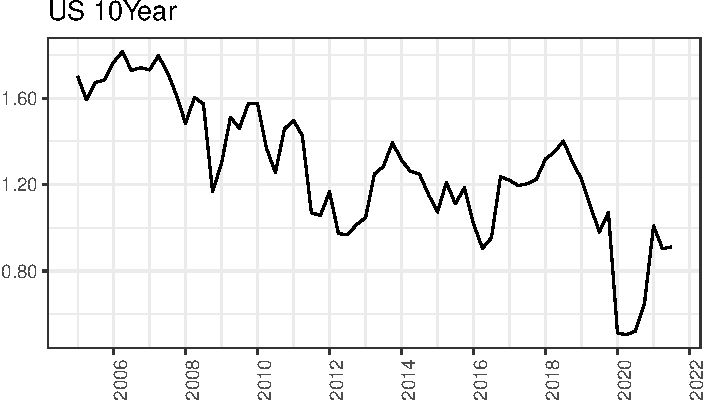
\includegraphics{Factor-Model_files/figure-latex/unnamed-chunk-1-1} \caption{US Long-Term Bond Yields}\label{fig:unnamed-chunk-1}
\end{figure}

\begin{figure}[H]
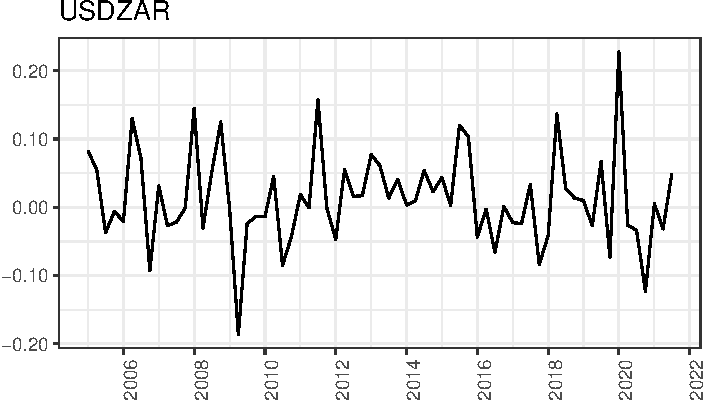
\includegraphics{Factor-Model_files/figure-latex/unnamed-chunk-2-1} \caption{USDZAR Spot Price}\label{fig:unnamed-chunk-2}
\end{figure}

\begin{figure}[H]
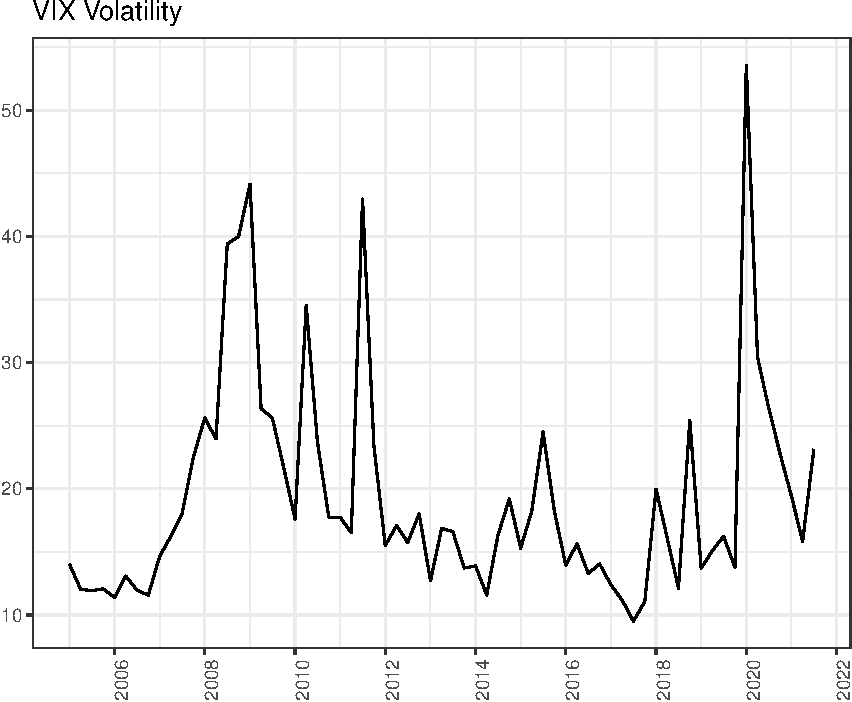
\includegraphics{Factor-Model_files/figure-latex/unnamed-chunk-3-1} \caption{CBOE VIX Volatility Index}\label{fig:unnamed-chunk-3}
\end{figure}

\begin{figure}[H]
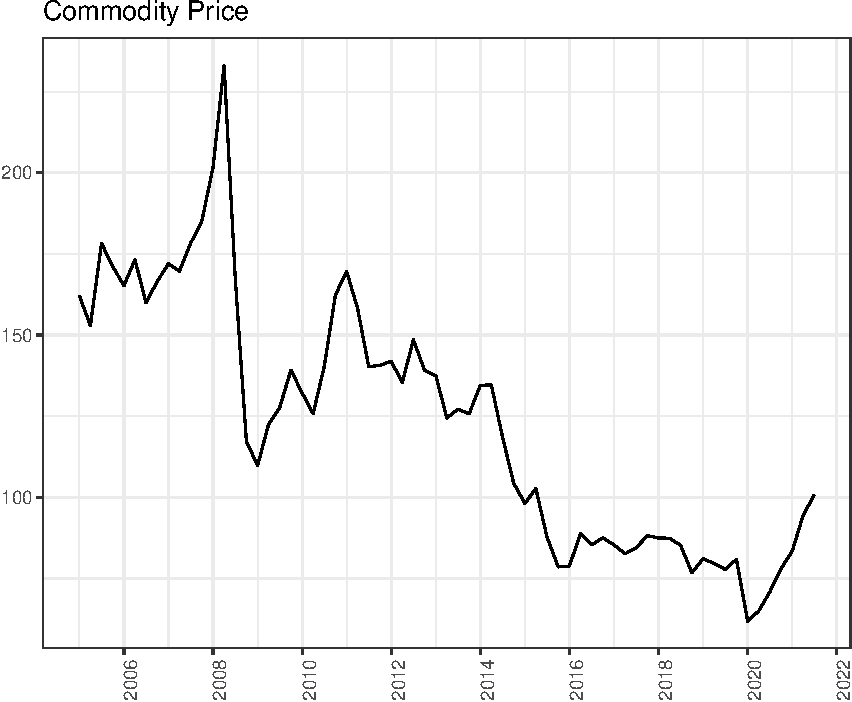
\includegraphics{Factor-Model_files/figure-latex/unnamed-chunk-4-1} \caption{Bloomberg Commodity Price Index}\label{fig:unnamed-chunk-4}
\end{figure}

\begin{figure}[H]
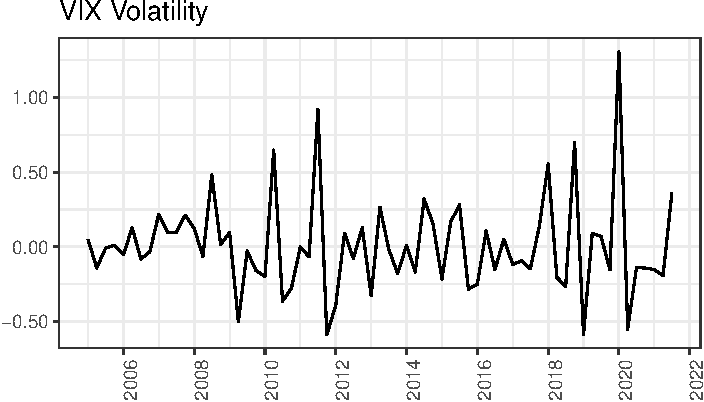
\includegraphics{Factor-Model_files/figure-latex/unnamed-chunk-5-1} \caption{South Africa Money Market Rate}\label{fig:unnamed-chunk-5}
\end{figure}

\begin{figure}[H]
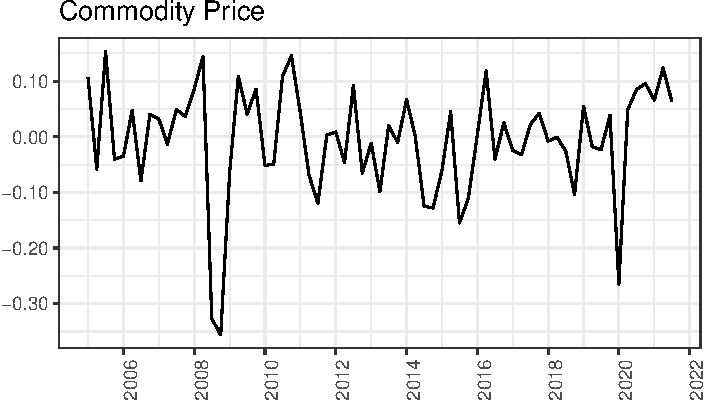
\includegraphics{Factor-Model_files/figure-latex/unnamed-chunk-6-1} \caption{South Africa Real GDP}\label{fig:unnamed-chunk-6}
\end{figure}

\begin{figure}[H]
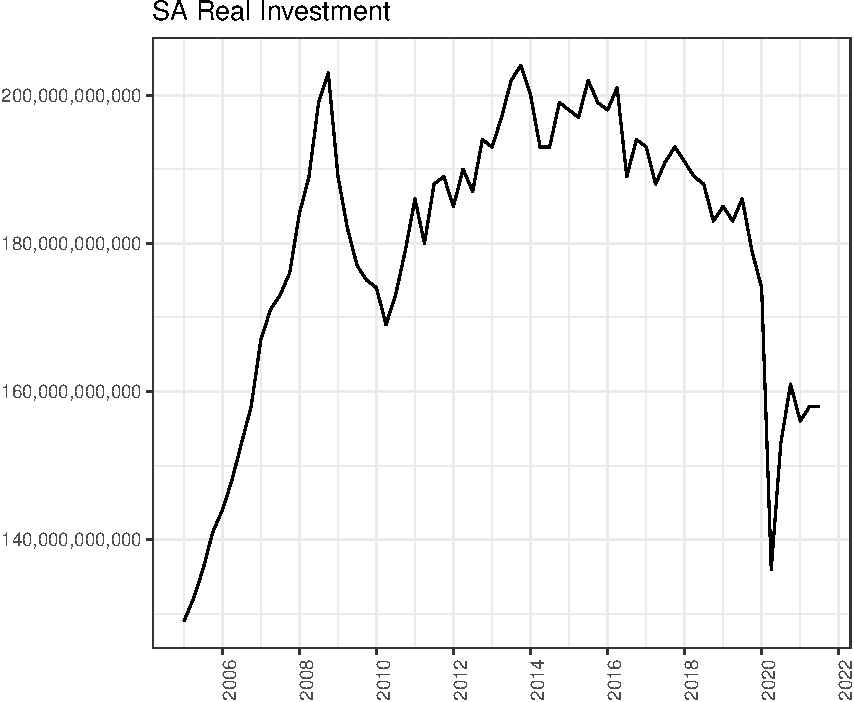
\includegraphics{Factor-Model_files/figure-latex/unnamed-chunk-7-1} \caption{South Africa Real Gross Fixed Capital Formation}\label{fig:unnamed-chunk-7}
\end{figure}

\begin{figure}[H]
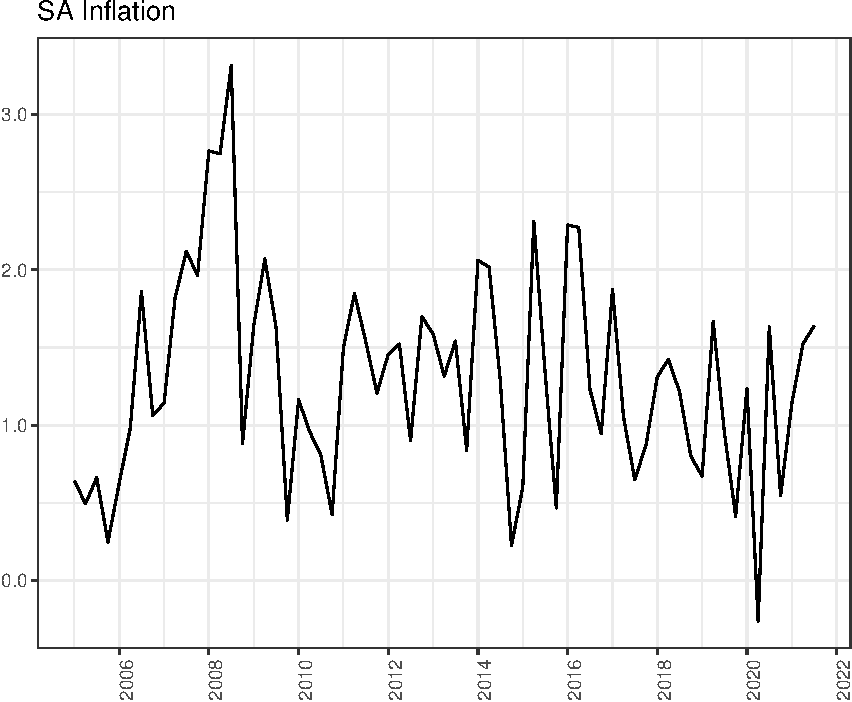
\includegraphics{Factor-Model_files/figure-latex/unnamed-chunk-8-1} \caption{South Africa Consumer Price Inflation}\label{fig:unnamed-chunk-8}
\end{figure}

\begin{figure}[H]
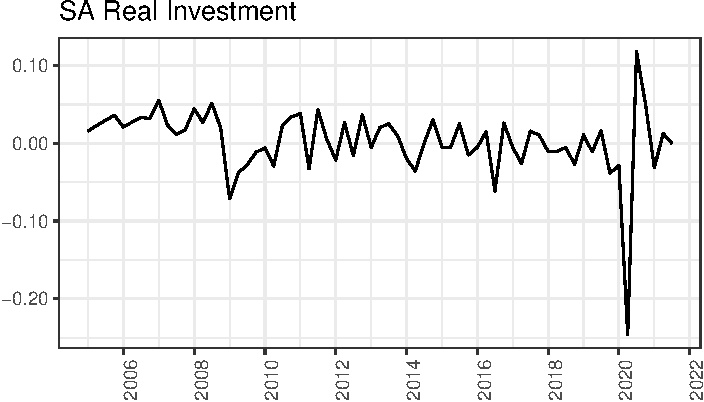
\includegraphics{Factor-Model_files/figure-latex/unnamed-chunk-9-1} \caption{Asset Returns by Industry}\label{fig:unnamed-chunk-9}
\end{figure}

\hypertarget{empirical-analysis}{%
\section{Empirical Analysis}\label{empirical-analysis}}

\hypertarget{methodology}{%
\subsection{Methodology}\label{methodology}}

\hypertarget{model-estimation-by-industry}{%
\subsection{Model Estimation (by
Industry)}\label{model-estimation-by-industry}}

\begin{figure}[H]
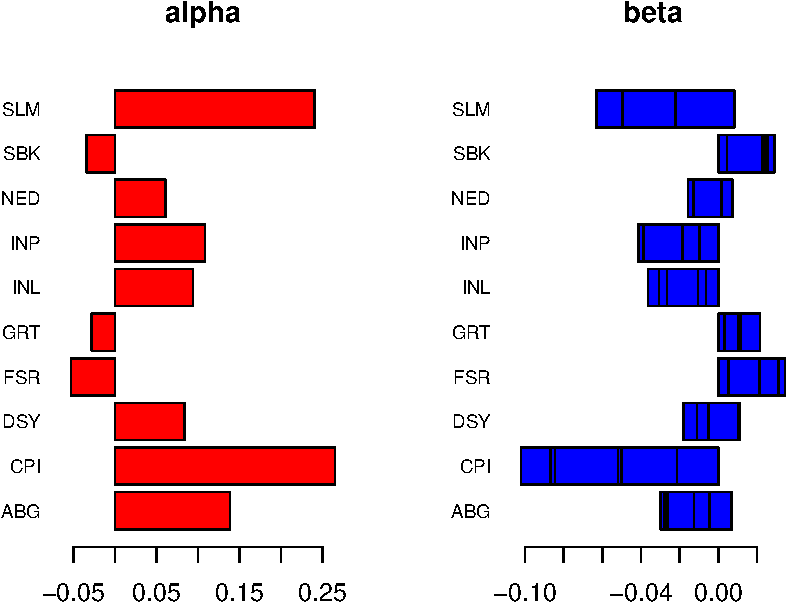
\includegraphics{Factor-Model_files/figure-latex/unnamed-chunk-10-1} \caption{Factor Analysis: Financials}\label{fig:unnamed-chunk-10}
\end{figure}

\begin{figure}[H]
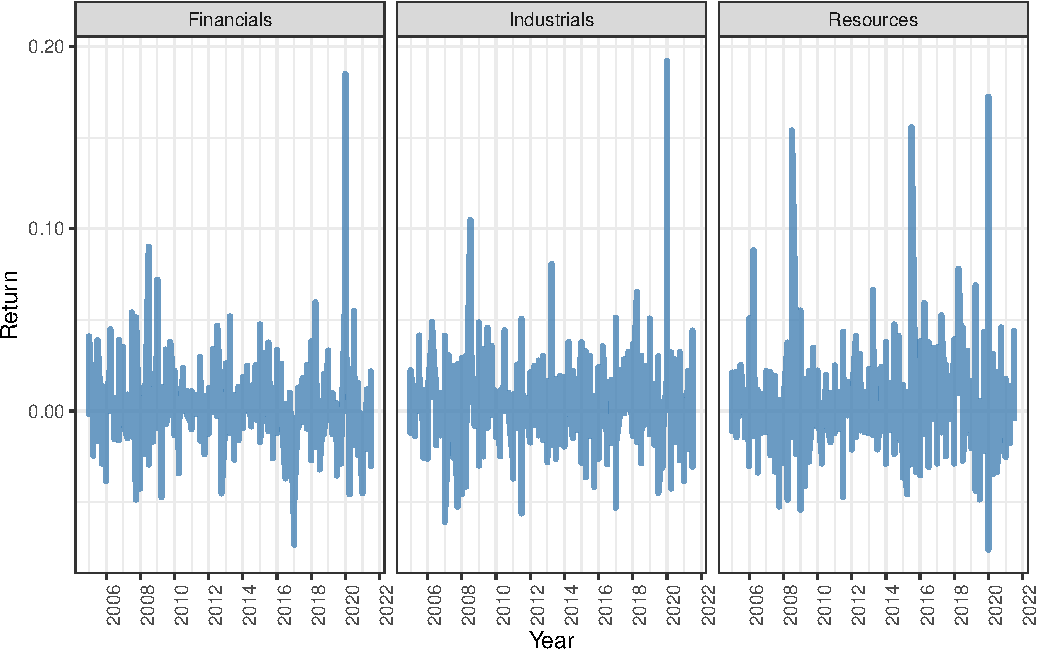
\includegraphics{Factor-Model_files/figure-latex/unnamed-chunk-11-1} \caption{Factor Analysis: Industrial}\label{fig:unnamed-chunk-11}
\end{figure}

\begin{figure}[H]
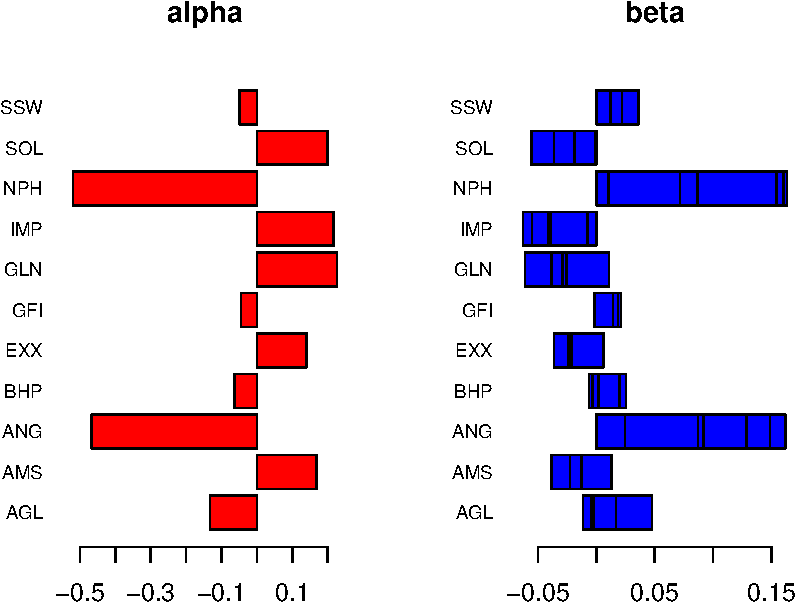
\includegraphics{Factor-Model_files/figure-latex/unnamed-chunk-12-1} \caption{Factor Analysis: Resources}\label{fig:unnamed-chunk-12}
\end{figure}

\hypertarget{discussion-of-results}{%
\subsection{Discussion of Results}\label{discussion-of-results}}

\hypertarget{conclusion}{%
\section{Conclusion}\label{conclusion}}

\newpage

\hypertarget{references}{%
\section{References}\label{references}}

\hypertarget{refs}{}
\begin{CSLReferences}{1}{0}
\leavevmode\hypertarget{ref-fama1997}{}%
Fama, E.F. \& French, K.R. 1997. Industry costs of equity. \emph{Journal
of financial economics}. 43(2):153--193.

\leavevmode\hypertarget{ref-Flannery}{}%
Flannery, M. \& Protopapadakis, A.A. 2002. Macroeconomic factors do
influence aggregate stock returns. \emph{Review of Financial Studies}.
15(3):751--782.

\leavevmode\hypertarget{ref-grinold2000}{}%
Grinold, R.C. \& Kahn, R.N. 2000. Active portfolio management.

\end{CSLReferences}

\newpage

\hypertarget{appendices}{%
\section{Appendices}\label{appendices}}

To reference the plot above, add a ``\textbackslash label'\,' after the
caption in the chunk heading, as done above. Then reference the plot as
such: As can be seen, Figures \ref{Figure1} and \ref{Figure2} are
excellent, with Figure \ref{Figure2} being particularly aesthetically
pleasing due to its device setting of Tikz. The nice thing now is that
it correctly numbers all your figures (and sections or tables) and will
update if it moves. The links are also dynamic.

\footnote{This is an example of a footnote by the way. Something that
  should also not be overused.}

Equations should be written as such:

\begin{align}
\beta = \sum_{i = 1}^{\infty}\frac{\alpha^2}{\sigma_{t-1}^2} \label{eq1} \\
\int_{x = 1}^{\infty}x_{i} = 1 \notag
\end{align}

If you would like to see the equations as you type in Rmarkdown, use \$
symbols instead (see this for yourself by adjusted the equation):

\[
\beta = \sum_{i = 1}^{\infty}\frac{\alpha^2}{\sigma_{t-1}^2} \\
\int_{x = 1}^{\infty}x_{i} = 1
\]

Note again the reference to equation \ref{eq1}. Writing nice math
requires practice. Note I used a forward slashes to make a space in the
equations.

\begin{table}[H]
\centering
\begin{tabular}{rrrrrrrrrrrr}
  \hline
 & mpg & cyl & disp & hp & drat & wt & qsec & vs & am & gear & carb \\ 
  \hline
1 & 21.00 & 6.00 & 160.00 & 110.00 & 3.90 & 2.62 & 16.46 & 0.00 & 1.00 & 4.00 & 4.00 \\ 
  2 & 21.00 & 6.00 & 160.00 & 110.00 & 3.90 & 2.88 & 17.02 & 0.00 & 1.00 & 4.00 & 4.00 \\ 
  3 & 22.80 & 4.00 & 108.00 & 93.00 & 3.85 & 2.32 & 18.61 & 1.00 & 1.00 & 4.00 & 1.00 \\ 
  4 & 21.40 & 6.00 & 258.00 & 110.00 & 3.08 & 3.21 & 19.44 & 1.00 & 0.00 & 3.00 & 1.00 \\ 
  5 & 18.70 & 8.00 & 360.00 & 175.00 & 3.15 & 3.44 & 17.02 & 0.00 & 0.00 & 3.00 & 2.00 \\ 
   \hline
\end{tabular}
\caption{Short Table Example \label{tab1}} 
\end{table}

To reference calculations \textbf{in text}, \emph{do this:} From table
\ref{tab1} we see the average value of mpg is 20.98.

Including tables that span across pages, use the following (note that I
add below the table: ``continue on the next page'\,'). This is a neat
way of splitting your table across a page.

Use the following default settings to build your own possibly long
tables. Note that the following will fit on one page if it can, but
cleanly spreads over multiple pages:

\begingroup\fontsize{12pt}{13pt}\selectfont
\begin{longtable}{rrrrrrrrrrr}
\caption{Long Table Example} \\ 
  \toprule
mpg & cyl & disp & hp & drat & wt & qsec & vs & am & gear & carb \\ 
  \hline 
\endhead 
\hline 
{\footnotesize Continued on next page} 
\endfoot 
\endlastfoot 
 \midrule
21.00 & 6.00 & 160.00 & 110.00 & 3.90 & 2.62 & 16.46 & 0.00 & 1.00 & 4.00 & 4.00 \\ 
  21.00 & 6.00 & 160.00 & 110.00 & 3.90 & 2.88 & 17.02 & 0.00 & 1.00 & 4.00 & 4.00 \\ 
  22.80 & 4.00 & 108.00 & 93.00 & 3.85 & 2.32 & 18.61 & 1.00 & 1.00 & 4.00 & 1.00 \\ 
  21.40 & 6.00 & 258.00 & 110.00 & 3.08 & 3.21 & 19.44 & 1.00 & 0.00 & 3.00 & 1.00 \\ 
  18.70 & 8.00 & 360.00 & 175.00 & 3.15 & 3.44 & 17.02 & 0.00 & 0.00 & 3.00 & 2.00 \\ 
  18.10 & 6.00 & 225.00 & 105.00 & 2.76 & 3.46 & 20.22 & 1.00 & 0.00 & 3.00 & 1.00 \\ 
  14.30 & 8.00 & 360.00 & 245.00 & 3.21 & 3.57 & 15.84 & 0.00 & 0.00 & 3.00 & 4.00 \\ 
  24.40 & 4.00 & 146.70 & 62.00 & 3.69 & 3.19 & 20.00 & 1.00 & 0.00 & 4.00 & 2.00 \\ 
  22.80 & 4.00 & 140.80 & 95.00 & 3.92 & 3.15 & 22.90 & 1.00 & 0.00 & 4.00 & 2.00 \\ 
  19.20 & 6.00 & 167.60 & 123.00 & 3.92 & 3.44 & 18.30 & 1.00 & 0.00 & 4.00 & 4.00 \\ 
  17.80 & 6.00 & 167.60 & 123.00 & 3.92 & 3.44 & 18.90 & 1.00 & 0.00 & 4.00 & 4.00 \\ 
  16.40 & 8.00 & 275.80 & 180.00 & 3.07 & 4.07 & 17.40 & 0.00 & 0.00 & 3.00 & 3.00 \\ 
  17.30 & 8.00 & 275.80 & 180.00 & 3.07 & 3.73 & 17.60 & 0.00 & 0.00 & 3.00 & 3.00 \\ 
  15.20 & 8.00 & 275.80 & 180.00 & 3.07 & 3.78 & 18.00 & 0.00 & 0.00 & 3.00 & 3.00 \\ 
  10.40 & 8.00 & 472.00 & 205.00 & 2.93 & 5.25 & 17.98 & 0.00 & 0.00 & 3.00 & 4.00 \\ 
  10.40 & 8.00 & 460.00 & 215.00 & 3.00 & 5.42 & 17.82 & 0.00 & 0.00 & 3.00 & 4.00 \\ 
  14.70 & 8.00 & 440.00 & 230.00 & 3.23 & 5.34 & 17.42 & 0.00 & 0.00 & 3.00 & 4.00 \\ 
  32.40 & 4.00 & 78.70 & 66.00 & 4.08 & 2.20 & 19.47 & 1.00 & 1.00 & 4.00 & 1.00 \\ 
  30.40 & 4.00 & 75.70 & 52.00 & 4.93 & 1.61 & 18.52 & 1.00 & 1.00 & 4.00 & 2.00 \\ 
  33.90 & 4.00 & 71.10 & 65.00 & 4.22 & 1.83 & 19.90 & 1.00 & 1.00 & 4.00 & 1.00 \\ 
  21.50 & 4.00 & 120.10 & 97.00 & 3.70 & 2.46 & 20.01 & 1.00 & 0.00 & 3.00 & 1.00 \\ 
  15.50 & 8.00 & 318.00 & 150.00 & 2.76 & 3.52 & 16.87 & 0.00 & 0.00 & 3.00 & 2.00 \\ 
  15.20 & 8.00 & 304.00 & 150.00 & 3.15 & 3.44 & 17.30 & 0.00 & 0.00 & 3.00 & 2.00 \\ 
  13.30 & 8.00 & 350.00 & 245.00 & 3.73 & 3.84 & 15.41 & 0.00 & 0.00 & 3.00 & 4.00 \\ 
  19.20 & 8.00 & 400.00 & 175.00 & 3.08 & 3.85 & 17.05 & 0.00 & 0.00 & 3.00 & 2.00 \\ 
  27.30 & 4.00 & 79.00 & 66.00 & 4.08 & 1.94 & 18.90 & 1.00 & 1.00 & 4.00 & 1.00 \\ 
  26.00 & 4.00 & 120.30 & 91.00 & 4.43 & 2.14 & 16.70 & 0.00 & 1.00 & 5.00 & 2.00 \\ 
  30.40 & 4.00 & 95.10 & 113.00 & 3.77 & 1.51 & 16.90 & 1.00 & 1.00 & 5.00 & 2.00 \\ 
  15.80 & 8.00 & 351.00 & 264.00 & 4.22 & 3.17 & 14.50 & 0.00 & 1.00 & 5.00 & 4.00 \\ 
  19.70 & 6.00 & 145.00 & 175.00 & 3.62 & 2.77 & 15.50 & 0.00 & 1.00 & 5.00 & 6.00 \\ 
  15.00 & 8.00 & 301.00 & 335.00 & 3.54 & 3.57 & 14.60 & 0.00 & 1.00 & 5.00 & 8.00 \\ 
  21.40 & 4.00 & 121.00 & 109.00 & 4.11 & 2.78 & 18.60 & 1.00 & 1.00 & 4.00 & 2.00 \\ 
   \bottomrule
\end{longtable}
\endgroup

\hfill

Note that I do not include this in the ordinary template, as some latex
users have complained it breaks when they build their Rmds (especially
those using tidytex - I don't have this problem as I have the full
Miktex installed on mine). Up to you, but I strongly recommend
installing the package manually and using huxtable. To make this work,
uncomment the \emph{Adding additional latex packages} part in yaml at
the top of the Rmd file. Then comment out the huxtable example in the
template below this line. Reknit, and enjoy.

 
  \providecommand{\huxb}[2]{\arrayrulecolor[RGB]{#1}\global\arrayrulewidth=#2pt}
  \providecommand{\huxvb}[2]{\color[RGB]{#1}\vrule width #2pt}
  \providecommand{\huxtpad}[1]{\rule{0pt}{#1}}
  \providecommand{\huxbpad}[1]{\rule[-#1]{0pt}{#1}}

\begin{table}[ht]
\begin{centerbox}
\begin{threeparttable}
\captionsetup{justification=centering,singlelinecheck=off}
\caption{Regression Output}
 \label{Reg01}
\setlength{\tabcolsep}{0pt}
\begin{tabular}{l l l l}


\hhline{>{\huxb{0, 0, 0}{0.8}}->{\huxb{0, 0, 0}{0.8}}->{\huxb{0, 0, 0}{0.8}}->{\huxb{0, 0, 0}{0.8}}-}
\arrayrulecolor{black}

\multicolumn{1}{!{\huxvb{0, 0, 0}{0}}c!{\huxvb{0, 0, 0}{0}}}{\huxtpad{6pt + 1em}\centering \hspace{6pt} {\fontsize{12pt}{14.4pt}\selectfont } \hspace{6pt}\huxbpad{6pt}} &
\multicolumn{1}{c!{\huxvb{0, 0, 0}{0}}}{\huxtpad{6pt + 1em}\centering \hspace{6pt} {\fontsize{12pt}{14.4pt}\selectfont Reg1} \hspace{6pt}\huxbpad{6pt}} &
\multicolumn{1}{c!{\huxvb{0, 0, 0}{0}}}{\huxtpad{6pt + 1em}\centering \hspace{6pt} {\fontsize{12pt}{14.4pt}\selectfont Reg2} \hspace{6pt}\huxbpad{6pt}} &
\multicolumn{1}{c!{\huxvb{0, 0, 0}{0}}}{\huxtpad{6pt + 1em}\centering \hspace{6pt} {\fontsize{12pt}{14.4pt}\selectfont Reg3} \hspace{6pt}\huxbpad{6pt}} \tabularnewline[-0.5pt]


\hhline{>{\huxb{255, 255, 255}{0.4}}->{\huxb{0, 0, 0}{0.4}}->{\huxb{0, 0, 0}{0.4}}->{\huxb{0, 0, 0}{0.4}}-}
\arrayrulecolor{black}

\multicolumn{1}{!{\huxvb{0, 0, 0}{0}}l!{\huxvb{0, 0, 0}{0}}}{\huxtpad{6pt + 1em}\raggedright \hspace{6pt} {\fontsize{12pt}{14.4pt}\selectfont (Intercept)} \hspace{6pt}\huxbpad{6pt}} &
\multicolumn{1}{r!{\huxvb{0, 0, 0}{0}}}{\huxtpad{6pt + 1em}\raggedleft \hspace{6pt} {\fontsize{12pt}{14.4pt}\selectfont -2256.361 ***} \hspace{6pt}\huxbpad{6pt}} &
\multicolumn{1}{r!{\huxvb{0, 0, 0}{0}}}{\huxtpad{6pt + 1em}\raggedleft \hspace{6pt} {\fontsize{12pt}{14.4pt}\selectfont 5763.668 ***} \hspace{6pt}\huxbpad{6pt}} &
\multicolumn{1}{r!{\huxvb{0, 0, 0}{0}}}{\huxtpad{6pt + 1em}\raggedleft \hspace{6pt} {\fontsize{12pt}{14.4pt}\selectfont 4045.333 ***} \hspace{6pt}\huxbpad{6pt}} \tabularnewline[-0.5pt]


\hhline{}
\arrayrulecolor{black}

\multicolumn{1}{!{\huxvb{0, 0, 0}{0}}l!{\huxvb{0, 0, 0}{0}}}{\huxtpad{6pt + 1em}\raggedright \hspace{6pt} {\fontsize{12pt}{14.4pt}\selectfont } \hspace{6pt}\huxbpad{6pt}} &
\multicolumn{1}{r!{\huxvb{0, 0, 0}{0}}}{\huxtpad{6pt + 1em}\raggedleft \hspace{6pt} {\fontsize{12pt}{14.4pt}\selectfont (13.055)\hphantom{0}\hphantom{0}\hphantom{0}} \hspace{6pt}\huxbpad{6pt}} &
\multicolumn{1}{r!{\huxvb{0, 0, 0}{0}}}{\huxtpad{6pt + 1em}\raggedleft \hspace{6pt} {\fontsize{12pt}{14.4pt}\selectfont (740.556)\hphantom{0}\hphantom{0}\hphantom{0}} \hspace{6pt}\huxbpad{6pt}} &
\multicolumn{1}{r!{\huxvb{0, 0, 0}{0}}}{\huxtpad{6pt + 1em}\raggedleft \hspace{6pt} {\fontsize{12pt}{14.4pt}\selectfont (286.205)\hphantom{0}\hphantom{0}\hphantom{0}} \hspace{6pt}\huxbpad{6pt}} \tabularnewline[-0.5pt]


\hhline{}
\arrayrulecolor{black}

\multicolumn{1}{!{\huxvb{0, 0, 0}{0}}l!{\huxvb{0, 0, 0}{0}}}{\huxtpad{6pt + 1em}\raggedright \hspace{6pt} {\fontsize{12pt}{14.4pt}\selectfont carat} \hspace{6pt}\huxbpad{6pt}} &
\multicolumn{1}{r!{\huxvb{0, 0, 0}{0}}}{\huxtpad{6pt + 1em}\raggedleft \hspace{6pt} {\fontsize{12pt}{14.4pt}\selectfont 7756.426 ***} \hspace{6pt}\huxbpad{6pt}} &
\multicolumn{1}{r!{\huxvb{0, 0, 0}{0}}}{\huxtpad{6pt + 1em}\raggedleft \hspace{6pt} {\fontsize{12pt}{14.4pt}\selectfont \hphantom{0}\hphantom{0}\hphantom{0}\hphantom{0}\hphantom{0}\hphantom{0}\hphantom{0}\hphantom{0}} \hspace{6pt}\huxbpad{6pt}} &
\multicolumn{1}{r!{\huxvb{0, 0, 0}{0}}}{\huxtpad{6pt + 1em}\raggedleft \hspace{6pt} {\fontsize{12pt}{14.4pt}\selectfont 7765.141 ***} \hspace{6pt}\huxbpad{6pt}} \tabularnewline[-0.5pt]


\hhline{}
\arrayrulecolor{black}

\multicolumn{1}{!{\huxvb{0, 0, 0}{0}}l!{\huxvb{0, 0, 0}{0}}}{\huxtpad{6pt + 1em}\raggedright \hspace{6pt} {\fontsize{12pt}{14.4pt}\selectfont } \hspace{6pt}\huxbpad{6pt}} &
\multicolumn{1}{r!{\huxvb{0, 0, 0}{0}}}{\huxtpad{6pt + 1em}\raggedleft \hspace{6pt} {\fontsize{12pt}{14.4pt}\selectfont (14.067)\hphantom{0}\hphantom{0}\hphantom{0}} \hspace{6pt}\huxbpad{6pt}} &
\multicolumn{1}{r!{\huxvb{0, 0, 0}{0}}}{\huxtpad{6pt + 1em}\raggedleft \hspace{6pt} {\fontsize{12pt}{14.4pt}\selectfont \hphantom{0}\hphantom{0}\hphantom{0}\hphantom{0}\hphantom{0}\hphantom{0}\hphantom{0}\hphantom{0}} \hspace{6pt}\huxbpad{6pt}} &
\multicolumn{1}{r!{\huxvb{0, 0, 0}{0}}}{\huxtpad{6pt + 1em}\raggedleft \hspace{6pt} {\fontsize{12pt}{14.4pt}\selectfont (14.009)\hphantom{0}\hphantom{0}\hphantom{0}} \hspace{6pt}\huxbpad{6pt}} \tabularnewline[-0.5pt]


\hhline{}
\arrayrulecolor{black}

\multicolumn{1}{!{\huxvb{0, 0, 0}{0}}l!{\huxvb{0, 0, 0}{0}}}{\huxtpad{6pt + 1em}\raggedright \hspace{6pt} {\fontsize{12pt}{14.4pt}\selectfont depth} \hspace{6pt}\huxbpad{6pt}} &
\multicolumn{1}{r!{\huxvb{0, 0, 0}{0}}}{\huxtpad{6pt + 1em}\raggedleft \hspace{6pt} {\fontsize{12pt}{14.4pt}\selectfont \hphantom{0}\hphantom{0}\hphantom{0}\hphantom{0}\hphantom{0}\hphantom{0}\hphantom{0}\hphantom{0}} \hspace{6pt}\huxbpad{6pt}} &
\multicolumn{1}{r!{\huxvb{0, 0, 0}{0}}}{\huxtpad{6pt + 1em}\raggedleft \hspace{6pt} {\fontsize{12pt}{14.4pt}\selectfont -29.650 *\hphantom{0}\hphantom{0}} \hspace{6pt}\huxbpad{6pt}} &
\multicolumn{1}{r!{\huxvb{0, 0, 0}{0}}}{\huxtpad{6pt + 1em}\raggedleft \hspace{6pt} {\fontsize{12pt}{14.4pt}\selectfont -102.165 ***} \hspace{6pt}\huxbpad{6pt}} \tabularnewline[-0.5pt]


\hhline{}
\arrayrulecolor{black}

\multicolumn{1}{!{\huxvb{0, 0, 0}{0}}l!{\huxvb{0, 0, 0}{0}}}{\huxtpad{6pt + 1em}\raggedright \hspace{6pt} {\fontsize{12pt}{14.4pt}\selectfont } \hspace{6pt}\huxbpad{6pt}} &
\multicolumn{1}{r!{\huxvb{0, 0, 0}{0}}}{\huxtpad{6pt + 1em}\raggedleft \hspace{6pt} {\fontsize{12pt}{14.4pt}\selectfont \hphantom{0}\hphantom{0}\hphantom{0}\hphantom{0}\hphantom{0}\hphantom{0}\hphantom{0}\hphantom{0}} \hspace{6pt}\huxbpad{6pt}} &
\multicolumn{1}{r!{\huxvb{0, 0, 0}{0}}}{\huxtpad{6pt + 1em}\raggedleft \hspace{6pt} {\fontsize{12pt}{14.4pt}\selectfont (11.990)\hphantom{0}\hphantom{0}\hphantom{0}} \hspace{6pt}\huxbpad{6pt}} &
\multicolumn{1}{r!{\huxvb{0, 0, 0}{0}}}{\huxtpad{6pt + 1em}\raggedleft \hspace{6pt} {\fontsize{12pt}{14.4pt}\selectfont (4.635)\hphantom{0}\hphantom{0}\hphantom{0}} \hspace{6pt}\huxbpad{6pt}} \tabularnewline[-0.5pt]


\hhline{>{\huxb{255, 255, 255}{0.4}}->{\huxb{0, 0, 0}{0.4}}->{\huxb{0, 0, 0}{0.4}}->{\huxb{0, 0, 0}{0.4}}-}
\arrayrulecolor{black}

\multicolumn{1}{!{\huxvb{0, 0, 0}{0}}l!{\huxvb{0, 0, 0}{0}}}{\huxtpad{6pt + 1em}\raggedright \hspace{6pt} {\fontsize{12pt}{14.4pt}\selectfont N} \hspace{6pt}\huxbpad{6pt}} &
\multicolumn{1}{r!{\huxvb{0, 0, 0}{0}}}{\huxtpad{6pt + 1em}\raggedleft \hspace{6pt} {\fontsize{12pt}{14.4pt}\selectfont 53940\hphantom{0}\hphantom{0}\hphantom{0}\hphantom{0}\hphantom{0}\hphantom{0}\hphantom{0}\hphantom{0}} \hspace{6pt}\huxbpad{6pt}} &
\multicolumn{1}{r!{\huxvb{0, 0, 0}{0}}}{\huxtpad{6pt + 1em}\raggedleft \hspace{6pt} {\fontsize{12pt}{14.4pt}\selectfont 53940\hphantom{0}\hphantom{0}\hphantom{0}\hphantom{0}\hphantom{0}\hphantom{0}\hphantom{0}\hphantom{0}} \hspace{6pt}\huxbpad{6pt}} &
\multicolumn{1}{r!{\huxvb{0, 0, 0}{0}}}{\huxtpad{6pt + 1em}\raggedleft \hspace{6pt} {\fontsize{12pt}{14.4pt}\selectfont 53940\hphantom{0}\hphantom{0}\hphantom{0}\hphantom{0}\hphantom{0}\hphantom{0}\hphantom{0}\hphantom{0}} \hspace{6pt}\huxbpad{6pt}} \tabularnewline[-0.5pt]


\hhline{}
\arrayrulecolor{black}

\multicolumn{1}{!{\huxvb{0, 0, 0}{0}}l!{\huxvb{0, 0, 0}{0}}}{\huxtpad{6pt + 1em}\raggedright \hspace{6pt} {\fontsize{12pt}{14.4pt}\selectfont R2} \hspace{6pt}\huxbpad{6pt}} &
\multicolumn{1}{r!{\huxvb{0, 0, 0}{0}}}{\huxtpad{6pt + 1em}\raggedleft \hspace{6pt} {\fontsize{12pt}{14.4pt}\selectfont 0.849\hphantom{0}\hphantom{0}\hphantom{0}\hphantom{0}} \hspace{6pt}\huxbpad{6pt}} &
\multicolumn{1}{r!{\huxvb{0, 0, 0}{0}}}{\huxtpad{6pt + 1em}\raggedleft \hspace{6pt} {\fontsize{12pt}{14.4pt}\selectfont 0.000\hphantom{0}\hphantom{0}\hphantom{0}\hphantom{0}} \hspace{6pt}\huxbpad{6pt}} &
\multicolumn{1}{r!{\huxvb{0, 0, 0}{0}}}{\huxtpad{6pt + 1em}\raggedleft \hspace{6pt} {\fontsize{12pt}{14.4pt}\selectfont 0.851\hphantom{0}\hphantom{0}\hphantom{0}\hphantom{0}} \hspace{6pt}\huxbpad{6pt}} \tabularnewline[-0.5pt]


\hhline{>{\huxb{0, 0, 0}{0.8}}->{\huxb{0, 0, 0}{0.8}}->{\huxb{0, 0, 0}{0.8}}->{\huxb{0, 0, 0}{0.8}}-}
\arrayrulecolor{black}

\multicolumn{4}{!{\huxvb{0, 0, 0}{0}}l!{\huxvb{0, 0, 0}{0}}}{\huxtpad{6pt + 1em}\raggedright \hspace{6pt} {\fontsize{12pt}{14.4pt}\selectfont  *** p $<$ 0.001;  ** p $<$ 0.01;  * p $<$ 0.05.} \hspace{6pt}\huxbpad{6pt}} \tabularnewline[-0.5pt]


\hhline{}
\arrayrulecolor{black}
\end{tabular}
\end{threeparttable}\par\end{centerbox}

\end{table}
 

\bibliography{Tex/ref}





\end{document}
